
%%%%%%%%%%%%%%%%%%%% Frame Here %%%%%%%%%%%%%%%%%%%%%%%%%%%%%%%%%%%%%%%%%%%%%%%%
\begin{frame}[label=TitlePage_1]
\maketitle% first slide with title/author information
\end{frame}
%%%%%%%%%%%%%%%%%%%% Frame Here %%%%%%%%%%%%%%%%%%%%%%%%%%%%%%%%%%%%%%%%%%%%%%%%


%%%%%%%%%%%%%%%%%%%% Frame Here %%%%%%%%%%%%%%%%%%%%%%%%%%%%%%%%%%%%%%%%%%%%%%%%
\begin{frame}[label=Introduction_1]
\frametitle{Presention layout}
\begin{itemize}
\item
This presentation is based upon Capital in the 21st century (Harvard University Press, March 2014)
\item
This book studies the global dynamics of income and wealth distribution since 18c in 20+ countries; I use historical data collected over the past 15 years with Atkinson, Saez, Postel-Vinay, Rosenthal, Alvaredo, Zucman, and 30+ others; I try to shift attention from rising income inequality to rising wealth inequality
\item
The book includes four parts:
\begin{itemize}
\item
Part 1. Income and capital
\item
Part 2. The dynamics of the capital/income ratio 
\item
Part 3. The structure of inequalities
\item
Part 4. Regulating capital in the 21st century
\end{itemize}
\item 
I will present some results from Parts 2 \& 3, focusing upon the long-run evolution of capital/income ratios and wealth concentration (\href{all graphs and series are available online}{http://piketty.pse.ens.fr/capital21c}.
\end{itemize}
\end{frame}
%%%%%%%%%%%%%%%%%%%% Frame Here %%%%%%%%%%%%%%%%%%%%%%%%%%%%%%%%%%%%%%%%%%%%%%%%


%%%%%%%%%%%%%%%%%%%% Frame Here %%%%%%%%%%%%%%%%%%%%%%%%%%%%%%%%%%%%%%%%%%%%%%%%
\begin{frame}[label=WTID]
\frametitle{The World Top Incomes Database}
\begin{figure}[t]
\begin{minipage}[b]{\textwidth}
\centering
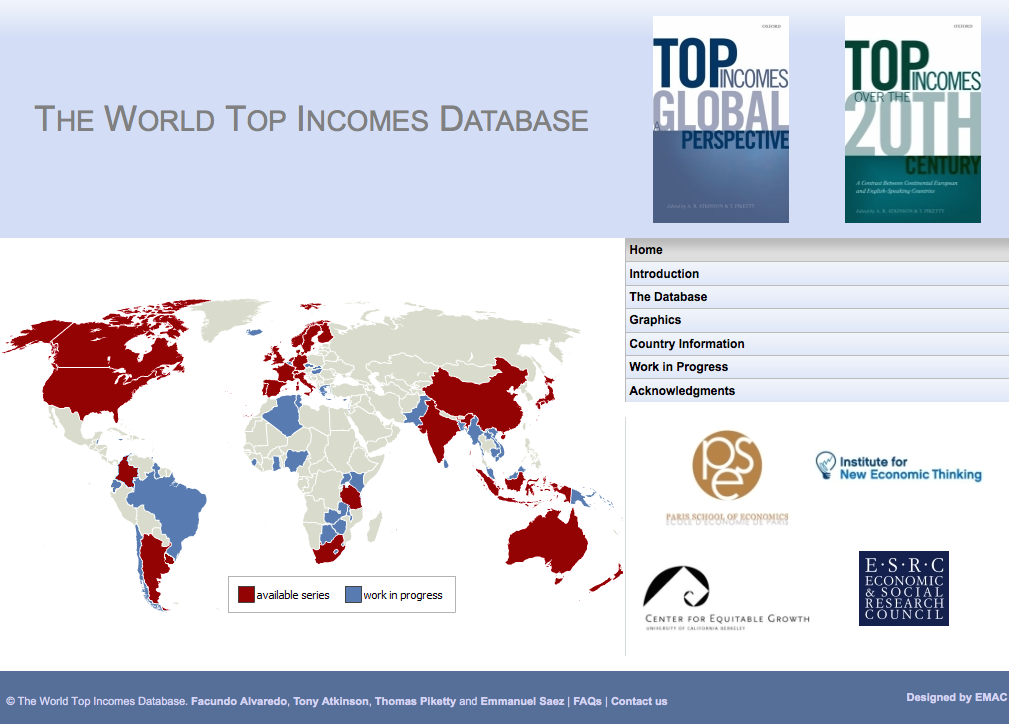
\includegraphics[width=0.9\textwidth]
{pictures/WorldTopIncomesDatabase}
\caption{\textbf{\url{http://topincomes.parisschoolofeconomics.eu}}}
\end{minipage}
\end{figure}
\end{frame}
%%%%%%%%%%%%%%%%%%%% Frame Here %%%%%%%%%%%%%%%%%%%%%%%%%%%%%%%%%%%%%%%%%%%%%%%%


%%%%%%%%%%%%%%%%%%%% Frame Here %%%%%%%%%%%%%%%%%%%%%%%%%%%%%%%%%%%%%%%%%%%%%%%%
\begin{frame}[label=ThreePoints,fragile,shrink=4]
\frametitle{This presentation: three points}
\begin{enumerate}
\item
\textbf{The return of a patrimonial (or wealth-based) society} in the Old World (Europe, Japan). Wealth-income ratios seem to be returning to very high levels in low growth countries.
\medskip\newline
Intuition: in a slow-growth society, wealth accumulated in the past can naturally become very important. In the very long run, this can be relevant for the entire world.
\item 
\textbf{The future of wealth concentration}: with high $r-g$ during 21c ($r =$~`net-of-tax rate of return', $g =$~`growth rate'), then wealth inequality might reach or surpass 19c oligarchic levels; conversely, suitable institutions can allow to democratize wealth.
\item
\textbf{Inequality in America} (``meritocratic extremism''): is the New World developing a new inequality model that is based upon extreme labor income inequality more than upon wealth inequality? Is it more merit-based, or can it become the worst of all worlds?
\end{enumerate}
\end{frame}
%%%%%%%%%%%%%%%%%%%% Frame Here %%%%%%%%%%%%%%%%%%%%%%%%%%%%%%%%%%%%%%%%%%%%%%%%


%%%%%%%%%%%%%%%%%%%% Frame Here %%%%%%%%%%%%%%%%%%%%%%%%%%%%%%%%%%%%%%%%%%%%%%%%
\begin{frame}[label=BrasilVersus]
\frametitle{Brasil vs Europe--US--Japan}
\begin{itemize}
\item
\textbf{Top income shares}: income inequality is known to be high in Brasil; but it is probably underestimated (problem with household surveys); little access to fiscal data in Brasil.
\item 
\textbf{Wealth-income ratios}: probably a strong rise in Brasil (real estate prices), but we do not really know.
\item
\textbf{Wealth inequality}: probably very high, but we do not really know; no access to property tax and inheritance tax statistics.
\item
\textbf{Like other countries, Brasil needs more transparency about income and wealth}; progressive tax on income, inheritance and wealth would be a powerful way to produce information about how the different income and wealth groups are benefiting from growth.
\end{itemize}
\end{frame}
%%%%%%%%%%%%%%%%%%%% Frame Here %%%%%%%%%%%%%%%%%%%%%%%%%%%%%%%%%%%%%%%%%%%%%%%%


%%%%%%%%%%%%%%%%%%%% Frame Here %%%%%%%%%%%%%%%%%%%%%%%%%%%%%%%%%%%%%%%%%%%%%%%%
\begin{frame}[label=BrazilUSTop1]
\frametitle{Top 1\% income share: Brazil and United States, 2006--2012}
\begin{figure}[t]
\begin{minipage}[b]{\textwidth}
\centering
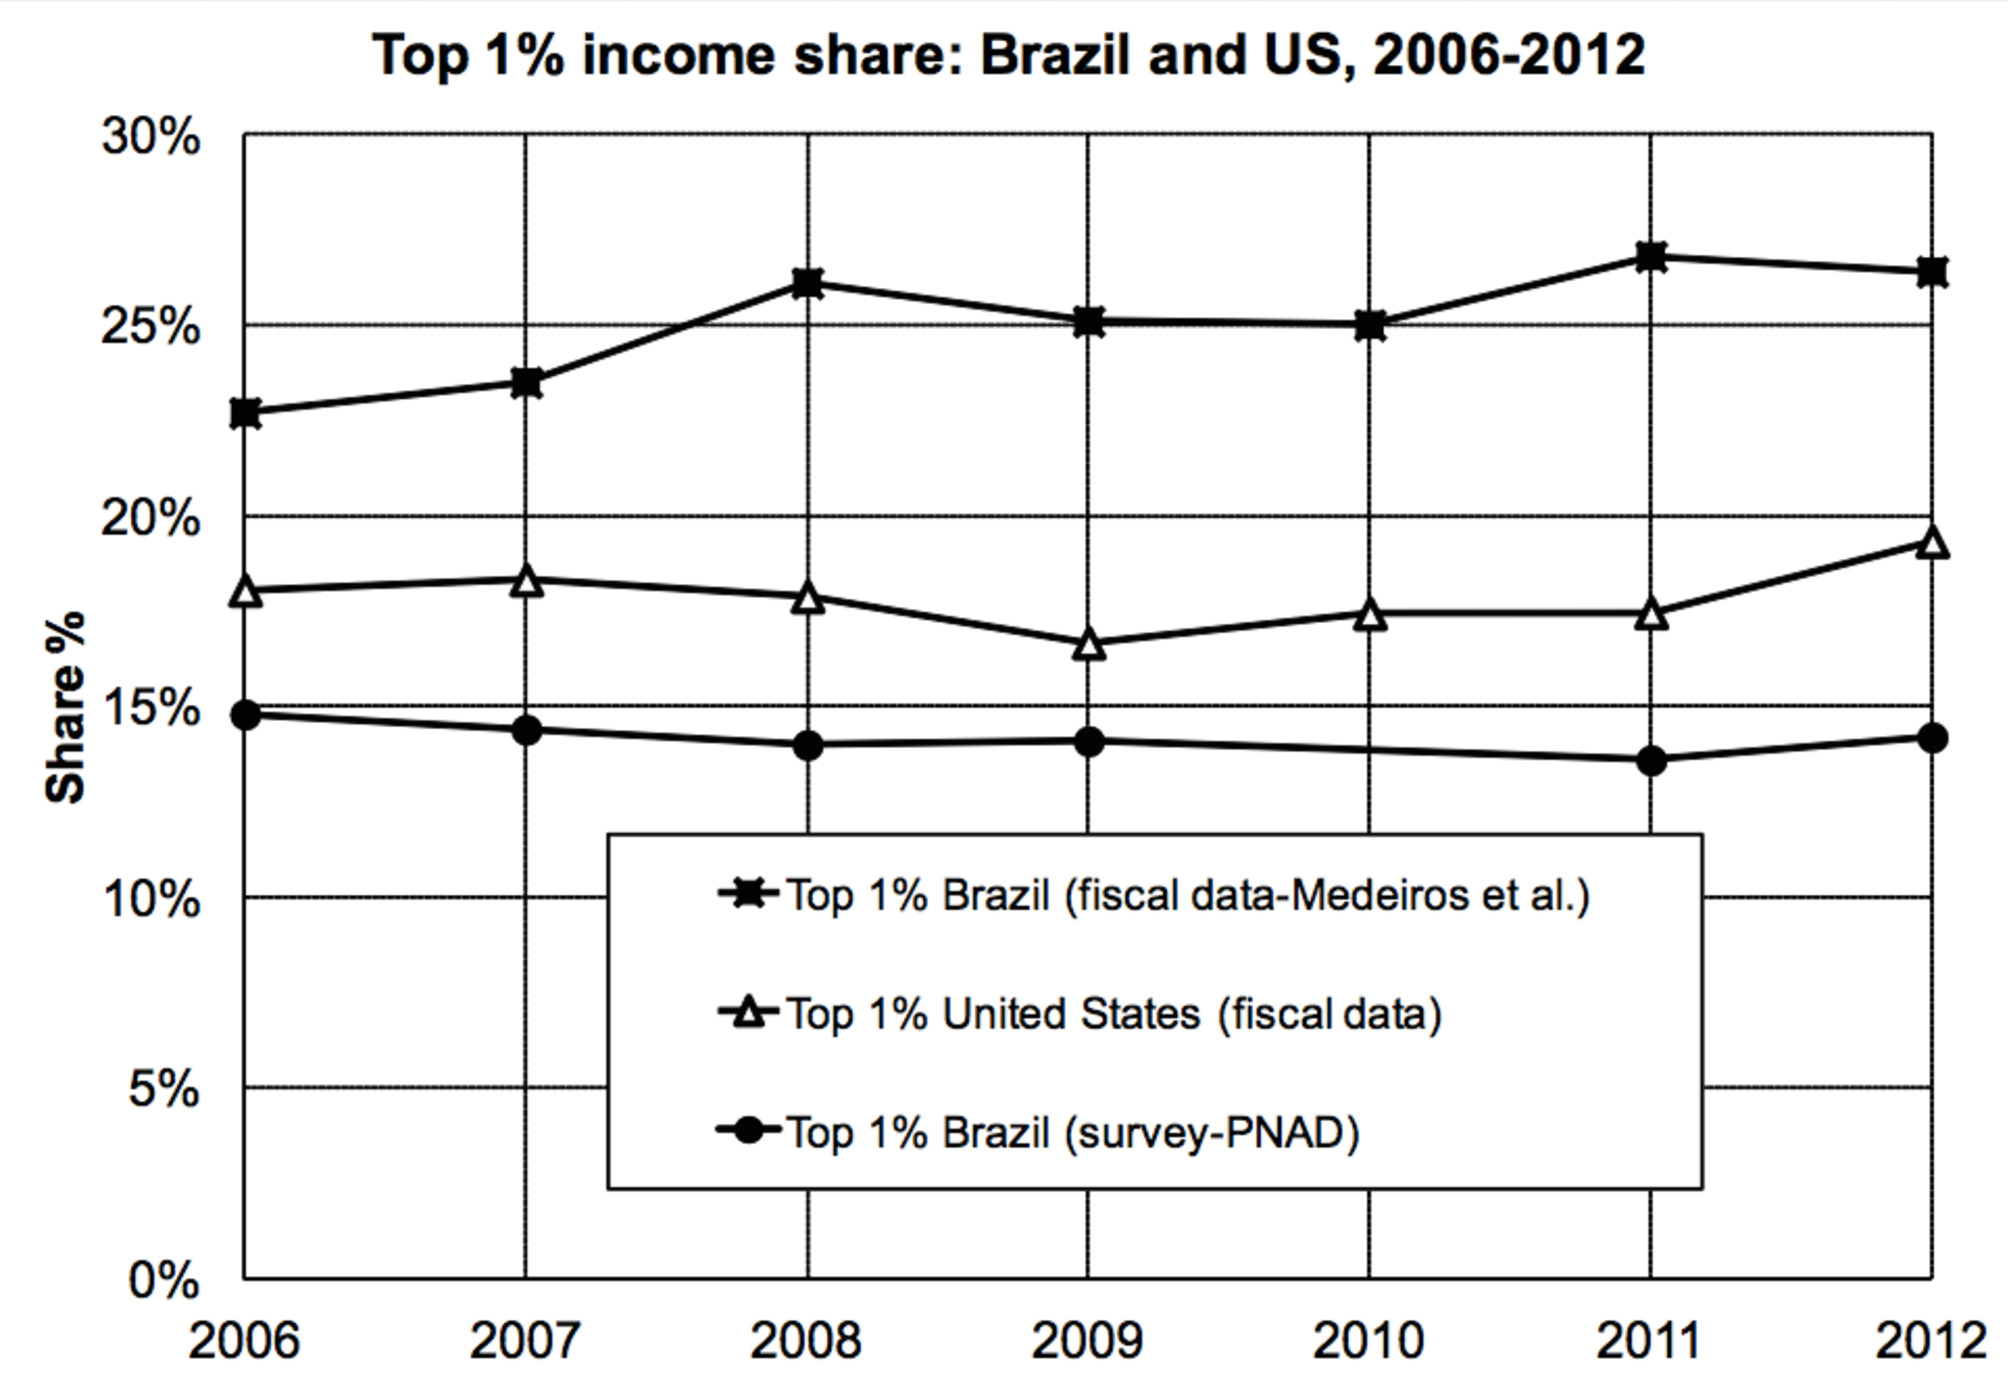
\includegraphics[width=\textwidth]
{pictures/Top1BrazilVsUSA}
\caption{To Do: Get Data to Recreate Figure}
\end{minipage}
\end{figure}
\end{frame}
%%%%%%%%%%%%%%%%%%%% Frame Here %%%%%%%%%%%%%%%%%%%%%%%%%%%%%%%%%%%%%%%%%%%%%%%%


%%%%%%%%%%%%%%%%%%%% Frame Here %%%%%%%%%%%%%%%%%%%%%%%%%%%%%%%%%%%%%%%%%%%%%%%%
\begin{frame}[label=BrazilUSTop10]
\frametitle{Top 10\% income share: Brazil and United States, 2006--2012}
\begin{figure}[t]
\begin{minipage}[b]{\textwidth}
\centering
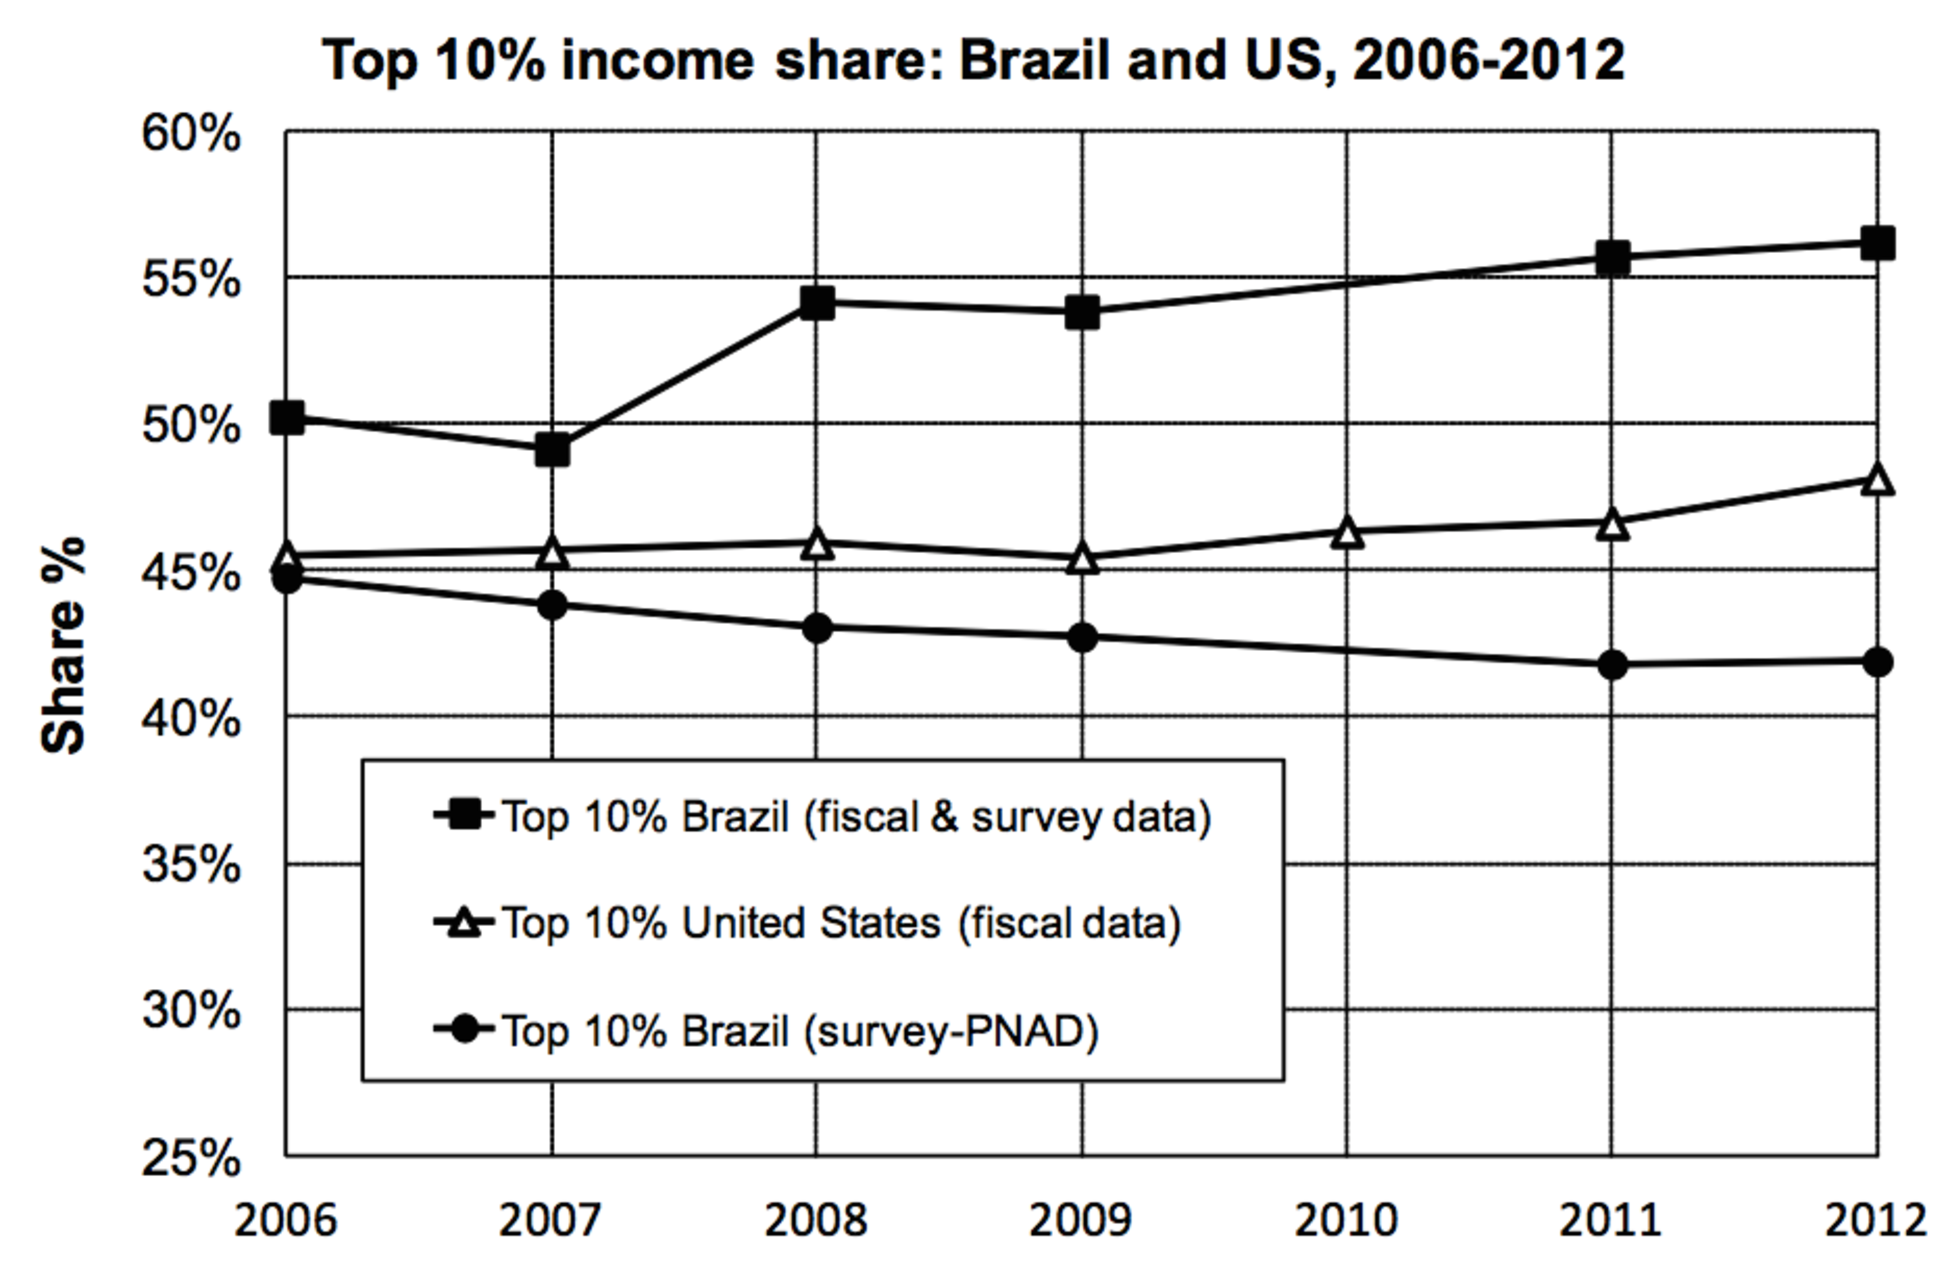
\includegraphics[width=\textwidth]
{pictures/Top10BrazilVsUSA}
\caption{To Do: Get Data to Recreate Figure}
\end{minipage}
\end{figure}
\end{frame}
%%%%%%%%%%%%%%%%%%%% Frame Here %%%%%%%%%%%%%%%%%%%%%%%%%%%%%%%%%%%%%%%%%%%%%%%%


%%%%%%%%%%%%%%%%%%%% Frame Here %%%%%%%%%%%%%%%%%%%%%%%%%%%%%%%%%%%%%%%%%%%%%%%%
\begin{frame}[label=BrazilInequality]
\frametitle{Income Inequality in Brazil: 1976--2013}
\begin{figure}[t]
\begin{minipage}[b]{\textwidth}
\centering
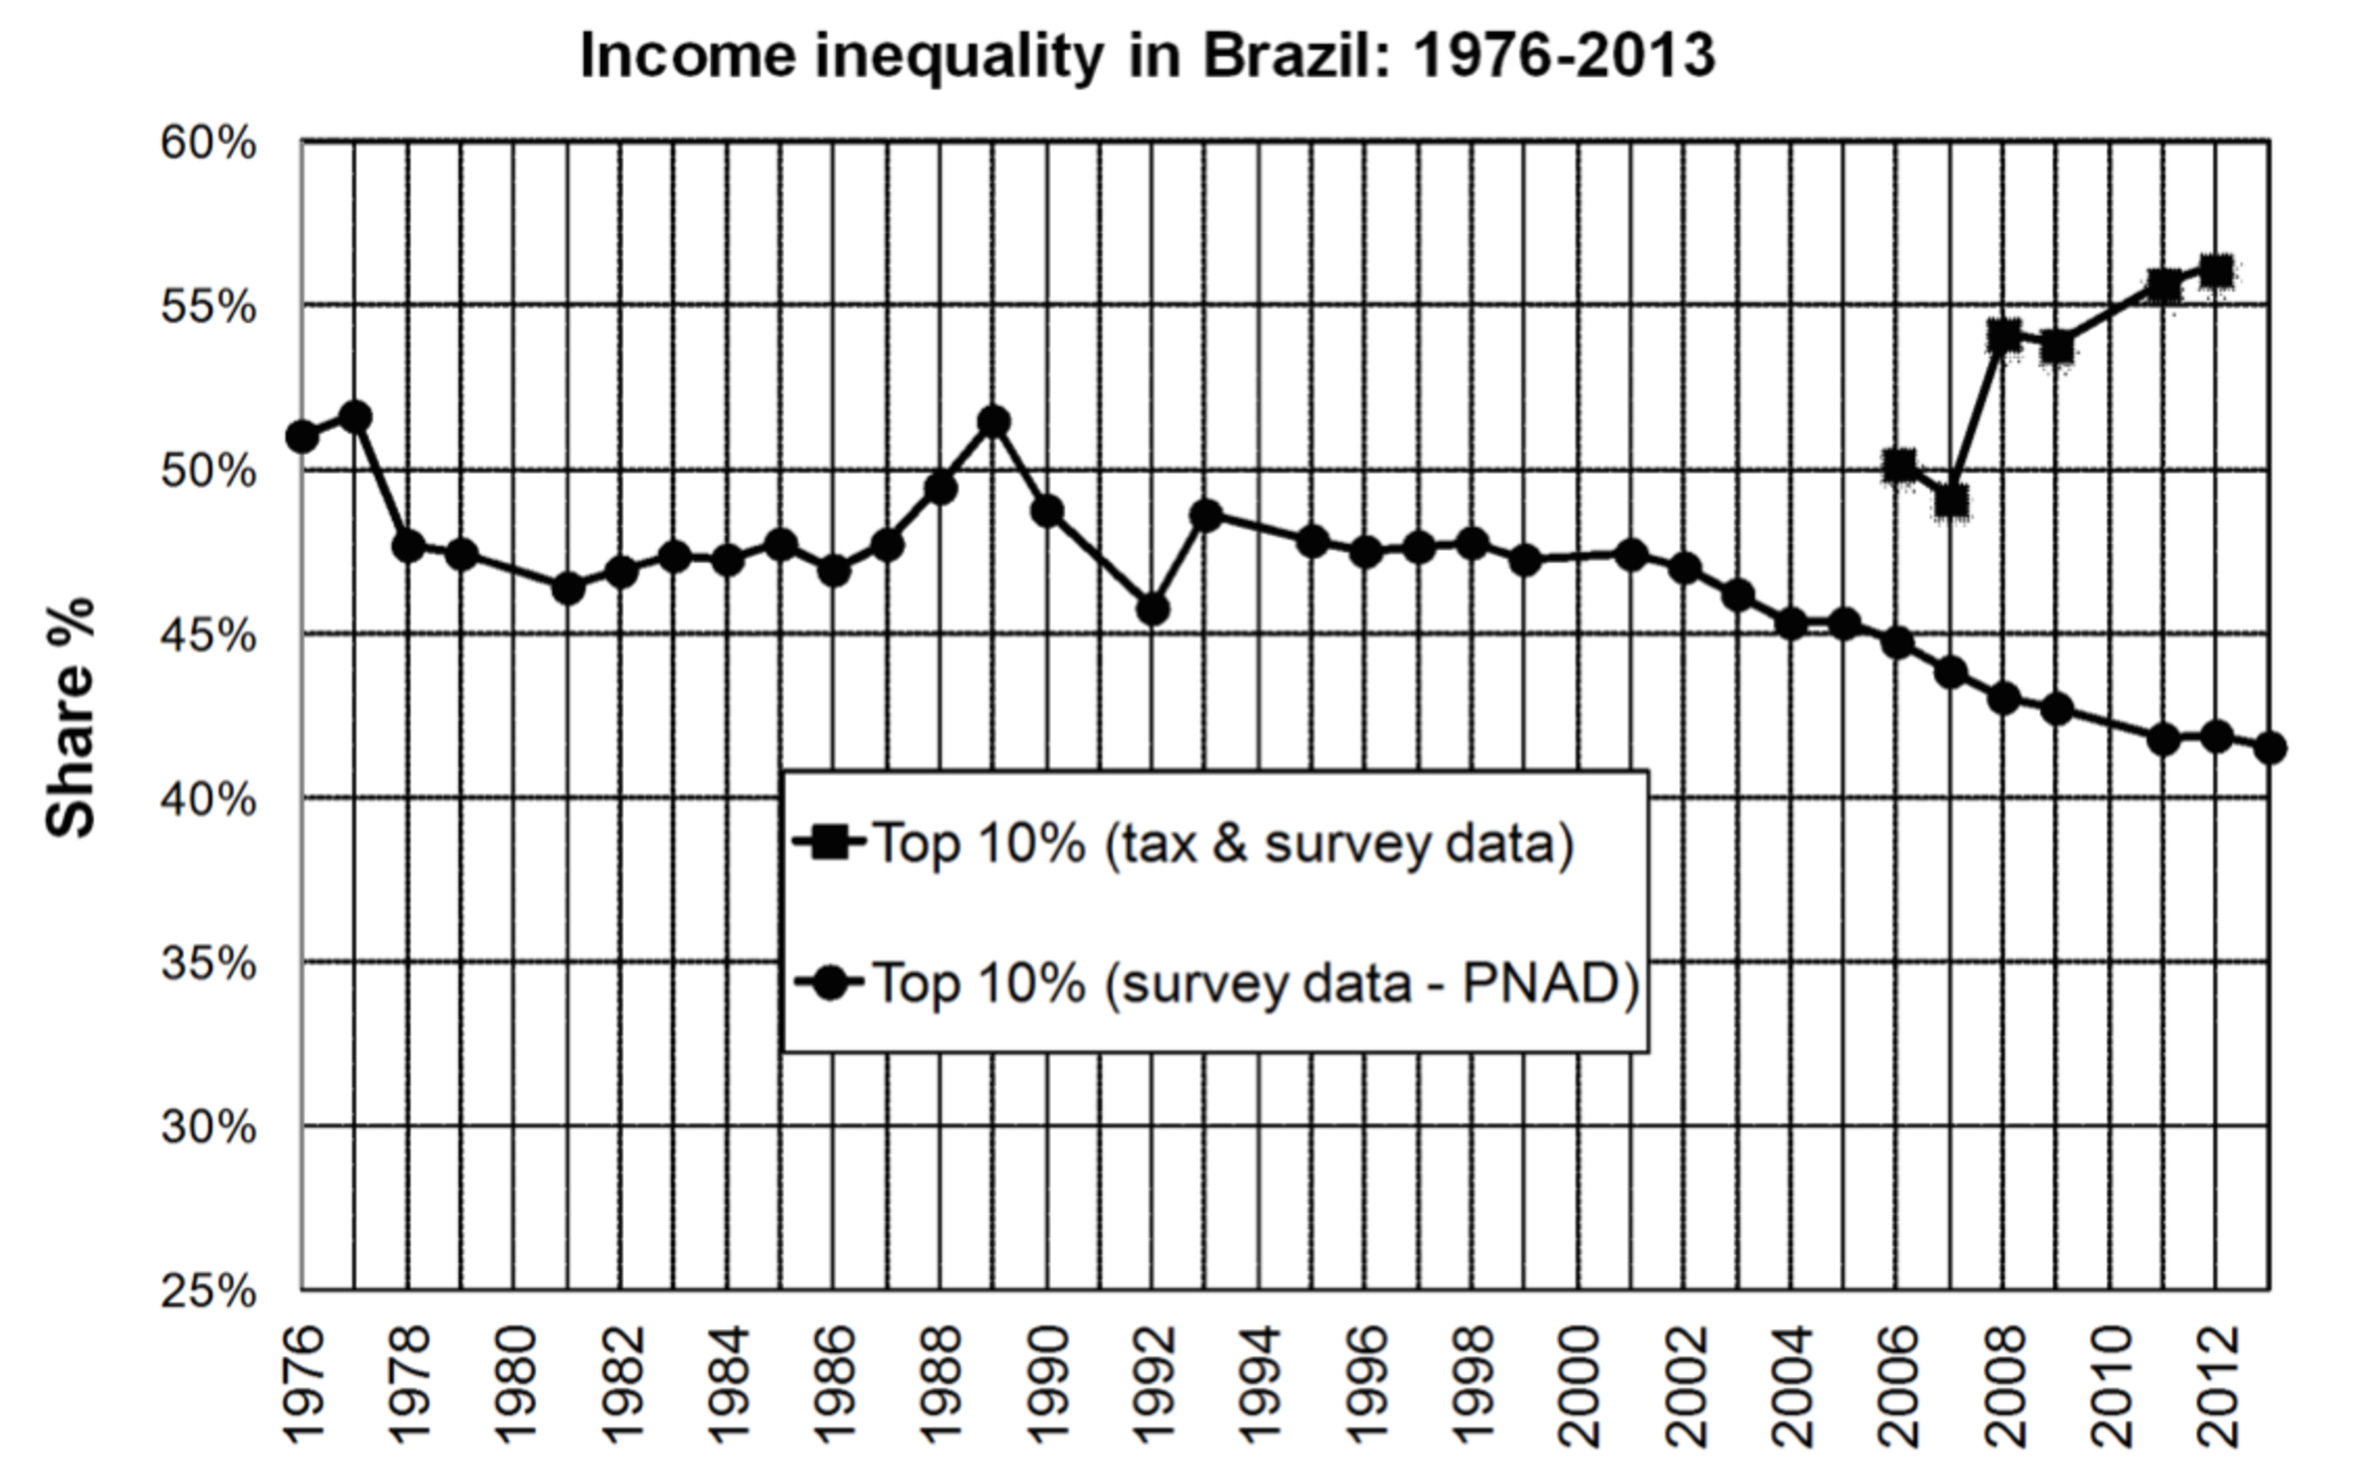
\includegraphics[width=\textwidth]
{pictures/IncomeInequalityBrazil}
\caption{To Do: Get Data to Recreate Figure}
\end{minipage}
\end{figure}
\end{frame}
%%%%%%%%%%%%%%%%%%%% Frame Here %%%%%%%%%%%%%%%%%%%%%%%%%%%%%%%%%%%%%%%%%%%%%%%%


%%%%%%%%%%%%%%%%%%%% Frame Here %%%%%%%%%%%%%%%%%%%%%%%%%%%%%%%%%%%%%%%%%%%%%%%%
\begin{frame}[label=Table_12_1]
\frametitle{Table 12.1: The growth rate of top global wealth, 1987--2013}
\begin{table}[t]
%\caption{The growth rate of top global wealth, 1987--2013}
\adjustbox{max height=\dimexpr\textheight-5.5cm\relax,
           max width=\textwidth}{%
\begin{threeparttable}
\centering
\begin{tabular}{@{}lc@{}}
\toprule
    & Average real growth rate per year  \\
    & (after deduction of inflation) (\%) \\
\midrule
    The top 1/(100 million) highest wealth holders \tnote{a}   & 6.8  \\
    The top 1/(20 million)  highest wealth holders \tnote{b}   & 6.4  \\
    Average world wealth per adult                             & 2.1  \\
    Average world income per adult                             & 1.4  \\
    World adult population                                     & 1.9  \\
    World GDP                                                  & 3.3  \\
\midrule
\end{tabular}
\begin{tablenotes}
    \item Between 1987 and 2013, the highest global wealth fractiles have grown at 6--7\% per year versus 2.1\% for average world wealth, and 1.4\% for average world income. All growth rates are net of inflation (2.3\% per year between 1987 and 2013).
    \item[a] About 30 adults out of 3 billion in the 1980s, and 45 adults out of 4.5 billion in 2010.
    \item[b] About 150 adults out of 3 billion in the 1980s, and 225 adults out of 4.5 billion in the 2010s.
\end{tablenotes}
\end{threeparttable}}
\end{table}
\end{frame}
%%%%%%%%%%%%%%%%%%%% Frame Here %%%%%%%%%%%%%%%%%%%%%%%%%%%%%%%%%%%%%%%%%%%%%%%%


%%%%%%%%%%%%%%%%%%%% Frame Here %%%%%%%%%%%%%%%%%%%%%%%%%%%%%%%%%%%%%%%%%%%%%%%%
\begin{frame}[label=Table_12_2]
\frametitle{Table 12.2: The return on the capital endowments of U.S. universities, 1980--2010}
\begin{table}[t]
%\caption{The return on the capital endowments of U.S. universities, 1980--2010}
\adjustbox{max height=\dimexpr\textheight-5.5cm\relax,
           max width=\textwidth}{%
\begin{threeparttable}
\centering
\begin{tabular}{@{}lc@{}}
\toprule
    & Average real annual rate of return                           \\
    & (after deduction of inflation and all                        \\
    & administrative costs and financial fees) (\%)                \\
\midrule
    All universities (850)                                & 8.2    \\
    Harvard, Yale, and Princeton                          & 10.2   \\
    Endowments higher than \$1 billion (60)               & 8.8    \\
    Endowments between \$500 million and 1 billion (66)   & 7.8    \\
    Endowments between \$100 and \$500 million (226)      & 7.1    \\
    Endowments less than \$100 million (498)              & 6.2    \\
\midrule
\end{tabular}
\begin{tablenotes}
    \item Between 1980 and 2010, U.S. universities earned an average real rate of return of 8.2\% on their capital endowments, and more for the greater endowments. All returns are reported net of inflation (2.4\% per year between 1980 and 2010) and net of administrative costs and financial fees.
\end{tablenotes}
\end{threeparttable}}
\end{table}
\end{frame}
%%%%%%%%%%%%%%%%%%%% Frame Here %%%%%%%%%%%%%%%%%%%%%%%%%%%%%%%%%%%%%%%%%%%%%%%%


%%%%%%%%%%%%%%%%%%%% Frame Here %%%%%%%%%%%%%%%%%%%%%%%%%%%%%%%%%%%%%%%%%%%%%%%%
\begin{frame}[label=Conclusions_1,shrink=7]
\frametitle{Conclusions}
\begin{itemize}
\item
\textbf{The history of income and wealth inequality is always political, chaotic and unpredictable; it involves national identities and sharp reversals; nobody can predict the reversals of the future.}
\item
Marx: with $g=0$, $\beta \to \infty$, $r \to 0$ : revolution, war
\item
My conclusions are less apocalyptic: with $g>0$, at least we have a steady state $\beta = s/g$.
\item
But with $g>0$ \& small, this steady-state can be rather gloomy: it can involve a very large capital-income ratio $\beta$ and capital share $\alpha$, as well as extreme wealth concentration due to high $r-g$.
\item
This has nothing to do with a market imperfection: the more perfect the capital market, the higher $r-g$.
\item
The ideal solution: progressive wealth tax at the global scale, based upon automatic exchange of bank information.
\item
Other solutions involve authoritarian political \& capital controls (China, Russia..), or perpetual population growth (US), or inflation, or some mixture of all.
\end{itemize}
\end{frame}
%%%%%%%%%%%%%%%%%%%% Frame Here %%%%%%%%%%%%%%%%%%%%%%%%%%%%%%%%%%%%%%%%%%%%%%%%


%%%%%%%%%%%%%%%%%%%% Frame Here %%%%%%%%%%%%%%%%%%%%%%%%%%%%%%%%%%%%%%%%%%%%%%%%
\begin{frame}[label=Transition_1]
\begin{center}
\begin{huge}
Supplementary Slides
\vspace{3\baselineskip}\par
(long lecture version)
\end{huge}
\end{center}
\end{frame}
%%%%%%%%%%%%%%%%%%%% Frame Here %%%%%%%%%%%%%%%%%%%%%%%%%%%%%%%%%%%%%%%%%%%%%%%%


% Long Version Starts Here


%%%%%%%%%%%%%%%%%%%% Frame Here %%%%%%%%%%%%%%%%%%%%%%%%%%%%%%%%%%%%%%%%%%%%%%%%
\begin{frame}[label=WealthReturn,shrink=8]
\frametitle{1. The return of a wealth-based society}
\begin{itemize}
\item
Wealth = capital $K$ = everything we own and that can be sold on a market (net of all debts) (excludes human $K$, except in slave societies)
\item
In textbooks, wealth-income \& capital-ouput ratios are supposed to be constant. But the so-called ``Kaldor facts'' actually rely on little historical evidence.
\item
In fact, we observe in Europe \& Japan a large recovery of $\beta=K/Y$ in recent decades:
\begin{align*}
\beta = 200-300\% ~\text{in}~ 1950-1960 \\
\beta = 500-600\% ~\text{in}~ 2000-2010
\end{align*}
\begin{footnotesize}
(i.e. average wealth $K$ was about 2--3 years of average income $Y$ around 1950--1960; it is about 5--6 years in 2000--2010)
\linebreak
(with $\beta \simeq 600\%$, if $Y \simeq \euro 30,000$ per capita, then $K \simeq \euro 180,000$ per capita) (currently, $K \simeq$ half real estate, half financial assets)
\end{footnotesize}
\item
\textbf{Are we heading back to the $\beta = 600-700\%$ observed in the wealth-based societies of 18c-19c? Or even more?}
\end{itemize}
\end{frame}
%%%%%%%%%%%%%%%%%%%% Frame Here %%%%%%%%%%%%%%%%%%%%%%%%%%%%%%%%%%%%%%%%%%%%%%%%


%%%%%%%%%%%%%%%%%%%% Frame Here %%%%%%%%%%%%%%%%%%%%%%%%%%%%%%%%%%%%%%%%%%%%%%%%
\begin{frame}[label=CapitalIsBack]
\frametitle{Capital is back}
\begin{itemize}
\item
The simplest way to think about this is the following: 
\begin{itemize}
\item
In the long-run, $\beta = s/g$
\par\medskip
with $s$ = (net-of-depreciation) saving rate and $g$ = economy's growth rate (population + productivity).
\end{itemize}
\item
With $s = 10\%$, $g = 3\%$, $\beta \simeq 300\%$; but if $s = 10\%$, $g = 1.5\%$, $\beta \simeq 600\%$.
\item
\textbf{In slow-growth societies, the total stock of wealth accumulated in the past can naturally be very important.}
\item
$\rightarrow$ \textbf{capital is back because low growth is back.}
(in particular because population growth $\downarrow 0$)
\item
$\rightarrow$ \textbf{in the long run, this can be relevant for the entire planet.}
\item
Note: $\beta = s/g$ = pure stock-flow accounting identity; it is true whatever the combination of saving motives.
\end{itemize}
\end{frame}
%%%%%%%%%%%%%%%%%%%% Frame Here %%%%%%%%%%%%%%%%%%%%%%%%%%%%%%%%%%%%%%%%%%%%%%%%


%%%%%%%%%%%%%%%%%%%% Frame Here %%%%%%%%%%%%%%%%%%%%%%%%%%%%%%%%%%%%%%%%%%%%%%%%
\begin{frame}[label=ElasticityKL,shrink=14]
\frametitle{The capital--labor elasticity of substitution}
\begin{itemize}
\item
\textbf{Will the rise of capital income-ratio $\beta$ also lead to a rise of the capital share $\alpha$ in national income?}
\item
If the capital stock equals $\beta = 6$ years of income and the average return to capital is equal $r = 5\%$ per year, then the share of capital income (rent, dividends, interest, profits, etc.) in national income equals $\alpha = r \times \beta = 30\%$.
\item
Technically, whether a rise in $\beta$ also leads to a rise in capital share $\alpha = r \beta$ depends on the elasticity of substitution $\sigma$ between capital $K$ and labor $L$ in the production function $Y = F(K, L)$.
\item
Intuition: $\sigma$ measures the extent to which workers can be replaced by machines (e.g. Amazon’s drones).
\item
Standard assumption: Cobb-Douglas production function ($\sigma = 1$) = as the stock $\beta \uparrow$, the return $r \downarrow$ exactly in the same proportions, so that $\alpha = r \times \beta$ remains unchanged, like by magic = a stable world where the capital--labor split is entirely set by technology.
\item
But if $\sigma > 1$, then the return to capital $r \downarrow$ falls less than the volume of capital $\beta\uparrow$, so that the product $\alpha = r \times \beta \uparrow$.
\item
\textbf{Exactly what happened since the 1970s--80s: both the ratio $\beta$ and the capital share $\alpha$ have increased.}
\end{itemize}
\end{frame}
%%%%%%%%%%%%%%%%%%%% Frame Here %%%%%%%%%%%%%%%%%%%%%%%%%%%%%%%%%%%%%%%%%%%%%%%%


%%%%%%%%%%%%%%%%%%%% Frame Here %%%%%%%%%%%%%%%%%%%%%%%%%%%%%%%%%%%%%%%%%%%%%%%%
\begin{frame}[label=Robots]
\frametitle{Towards a world of robots?}
\begin{itemize}
\item
With a large rise in $\beta$, one can get large rise in $\alpha$ with a production function $F(K,L)$ that is just a little bit more substituable than in the standard Cobb-Douglas model (say if $\sigma = 1.5$ instead of $1$).
\item
Maybe it is natural to expect $\sigma \uparrow$ over the course of history: more and more diversified uses for capital;
\textbf{extreme case: pure robot-economy} ($\sigma = $ infinity).
\item
Less extreme case: there are many possible uses for capital (machines can replace cashiers, drones can replace Amazon's delivery workers, etc.), so that the capital share $\alpha \uparrow$ continuously; there's no natural corrective mechanism for this.
\item
The rise of $\beta$ and $\alpha$ can be a good thing (we could all devote more time to culture, education, health..., rather than to our own subsistance), assuming one can answer the following question: \textbf{who owns the robots?}
\end{itemize}
\end{frame}
%%%%%%%%%%%%%%%%%%%% Frame Here %%%%%%%%%%%%%%%%%%%%%%%%%%%%%%%%%%%%%%%%%%%%%%%%


%%%%%%%%%%%%%%%%%%%% Frame Here %%%%%%%%%%%%%%%%%%%%%%%%%%%%%%%%%%%%%%%%%%%%%%%%
\begin{frame}[label=WealthFuture]
\frametitle{2. The future of wealth concentration}
\begin{itemize}
\item
In all European countries (UK, France, Sweden...), wealth concentration was extremely high in 18c-19c \& until WW1:
\begin{itemize}
\item
about 90\% of aggregate wealth for top 10\% wealth holders
\item
about 60\% of aggregate wealth for top 1\% wealth-holders
\end{itemize}
\item
\textbf{= the classic patrimonial (wealth-based) society}: 
\begin{itemize}
\item
a minority lives off its wealth, while the rest of the populaton works (Austen, Balzac)
\end{itemize}
\item
Today wealth concentration is still very high, but less extreme:\hfill
\begin{itemize}%\vspace{-\baselineskip}% hack
\item
about 60--70\% for top 10\%; about 20--30\% for top 1\%
\item
the bottom 50\% still owns almost nothing (<5\%)
\item
but the middle 40\% now owns 20--30\% of aggregate wealth
\item
\textbf{= the rise of a patrimonial middle class}.
\end{itemize}
\item
\textbf{How did it happen, and will it last? Will the patrimonial middle class expend, or will it shrink?}
\end{itemize}
\end{frame}
%%%%%%%%%%%%%%%%%%%% Frame Here %%%%%%%%%%%%%%%%%%%%%%%%%%%%%%%%%%%%%%%%%%%%%%%%


%%%%%%%%%%%%%%%%%%%% Frame Here %%%%%%%%%%%%%%%%%%%%%%%%%%%%%%%%%%%%%%%%%%%%%%%%
\begin{frame}[label=WealthShocks]
\frametitle{Wealth shocks}
\begin{itemize}
\item
\textbf{Key finding: there was no decline in wealth concentration prior to World War shocks; was it just due to shocks?}
\begin{itemize}
\item
\textbf{Question}: Apart from shocks, what forces determine the long-run level of wealth concentration?
\item
\textbf{Answer}: In any dynamic, multiplicative wealth accumulation model with random individual shocks (tastes, demographics, returns, wages,..), 
\textbf{the steady-state level of wealth concentration is an increasing function of $r-g$}. 
\smallskip\par (with $r$ = net-of-tax rate of return and $g$ = growth rate)
\end{itemize}
\item
With growth slowdown and rising tax competition to attract capital, $r-g$ might well rise in the 21c $\rightarrow$ back to 19c levels.
\item
Future values of $r$ also depend on technology ($\sigma > 1$?)
\item 
Under plausible assumptions, wealth concentration might reach or surpass 19c record levels: see global wealth rankings
\end{itemize}
\end{frame}
%%%%%%%%%%%%%%%%%%%% Frame Here %%%%%%%%%%%%%%%%%%%%%%%%%%%%%%%%%%%%%%%%%%%%%%%%


%%%%%%%%%%%%%%%%%%%% Frame Here %%%%%%%%%%%%%%%%%%%%%%%%%%%%%%%%%%%%%%%%%%%%%%%%
\begin{frame}[label=InequalityUSA]
\frametitle{3. Inequality in America}
\framesubtitle{``meritocratic extremism''}
\begin{itemize}
\item
Inequality in America = a different structure as in Europe: 
\textbf{more egalitarian in some ways, more inegalitarian in some other dimensions}.
\item
The New World in the 19th century: the land of opportunity (capital accumulated in the past mattered much less than in Europe; perpetual demographic growth as a way to reduce the level of inherited wealth and wealth concentration)... and also the land of slavery.
\item 
Northern US were in many ways more egalitarian than Old Europe; but Southern US were more inegalitarian.
\item 
We still have the same ambiguous relationship of America with inequality today: in some ways more merit-based; in other ways more violent (prisons).
\end{itemize}
\end{frame}
%%%%%%%%%%%%%%%%%%%% Frame Here %%%%%%%%%%%%%%%%%%%%%%%%%%%%%%%%%%%%%%%%%%%%%%%%


%%%%%%%%%%%%%%%%%%%% Frame Here %%%%%%%%%%%%%%%%%%%%%%%%%%%%%%%%%%%%%%%%%%%%%%%%
\begin{frame}[label=MeritVNorms]
\frametitle{Merit or Social Norms?}
\begin{itemize}
\item
Higher inequality of labor income in the US could reflect higher inequality in education investment; but it also reflects a huge rise of top executive compensation that it very hard to explain with education and productivity reasoning alone.
\item 
In the US, this is sometime described as more merit--based: the rise of top labor incomes makes it possible to become rich with no inheritance ($\simeq$~Napoleonic «préfets»)
\item 
\textbf{Problem: this can be the worst of all worlds for those who are neither top income earners nor top successors}: they are poor, and they are depicted as dump \& undeserving (by contrast, nobody was trying to depict Ancien Regime inequality as fair!).
\item 
It is unclear whether rise of top incomes has a lot to do with merit or productivity: sharp decline in top tax rates \& rise of CEO bargaining power are more convincing explanations; chaotic US history of social norms regarding inequality.
\end{itemize}
\end{frame}
%%%%%%%%%%%%%%%%%%%% Frame Here %%%%%%%%%%%%%%%%%%%%%%%%%%%%%%%%%%%%%%%%%%%%%%%%


